% Created 2023-07-26 Wed 11:36
% Intended LaTeX compiler: pdflatex
\documentclass[11pt]{article}
\usepackage[utf8]{inputenc}
\usepackage[T1]{fontenc}
\usepackage{graphicx}
\usepackage{longtable}
\usepackage{wrapfig}
\usepackage{rotating}
\usepackage[normalem]{ulem}
\usepackage{amsmath}
\usepackage{amssymb}
\usepackage{capt-of}
\usepackage{hyperref}
\usepackage{minted}
\usepackage[a4paper]{geometry}
\usepackage{mathtools}
\author{Alexander Huss}
\date{\today}
\title{Parton Showers}
\hypersetup{
 pdfauthor={Alexander Huss},
 pdftitle={Parton Showers},
 pdfkeywords={},
 pdfsubject={},
 pdfcreator={Emacs 28.2 (Org mode 9.7)}, 
 pdflang={English}}
\begin{document}

\maketitle
\tableofcontents



\section{Introduction}
\label{sec:org85d9fdd}
We will investigate the emission probability of gluons off quarks and gluons and use that to implement a \textbf{very} simplifued parton shower (only final state primary branching, leading double-log, only virtuality \(q^2\) and not proper kinematics, \ldots{}).

\section{Emission probability and the Sudakov form factor}
\label{sec:orga58c098}
In the leading double-log approximation (soft \emph{and} collinear emission), we have seen in the lecture that the emission propability is given as
\begin{align}
  \mathrm{d}\omega_{X\to X+g}
  &=
  2 \, \frac{\alpha_s}{\pi}\; C_X \; \frac{\mathrm{d}E}{E} \; \frac{\mathrm{d}\theta}{\theta}
  \,,
\end{align}
where \(E\) denotes the energy of the emitted gluon and \(\theta\) the angle w.r.t. the parent particle.
We denote the emitting particle by ``\(X\)'' and \(C_X\) is the associated colour factor.
For quarks, \(C_X=C_F=\tfrac{4}{3}\) and for gluons \(C_X=C_A=3\).

For any parton shower, we first need to fix the evolution variable w.r.t. which we want to generate emissions.
To this end, we choose the virtuality \(q^2\) associated with the emission for which we find
\begin{align}
  d\mathcal{P}
  &=
  \frac{\alpha_s}{\pi}\; C_X \; \frac{\mathrm{d}q^2}{q^2} \; \ln\biggl(\frac{q^2}{Q_0^2}\biggr)
\end{align}
where \(Q_0\) denotes a cutoff below which emissions are considered unresolved.
We next define the so-called Sudakov form factor \(\Delta(Q^2,q^2)\), which is the probability for \emph{no resolved emissions} to happen between \(Q^2 \to q^2\).
It saitisfies a differential equation reminiscent of radiative decay with a simple solution
\begin{align}
  \frac{\mathrm{d}\Delta(Q^2,q^2)}{\mathrm{d}q^2}
  &=
  \Delta(Q^2,q^2) \; \frac{\mathrm{d}\mathcal{P}}{\mathrm{d}q^2}
  \,,&
  \Delta(Q^2)
  &\equiv \Delta(Q^2,Q_0^2)
  =
  \exp\biggl\{-\frac{\alpha_s C_X}{2\pi} \, \ln^2\biggl(\frac{q^2}{Q_0^2}\biggr) \biggr\}
\end{align}

\section{Implementation}
\label{sec:org61bbcbf}

With the Sudakov form factor at hand, we can easily iterate the sampling of emissions using these steps:
\begin{enumerate}
\item set \(Q = Q_\mathrm{start}\)
\item draw a uniform random number \(r\) in the range \([0,\,1]\)
\item if \(r<\Delta(Q^2)\), no resolvable emission can be generated (\(<Q_0\)):
Terminate loop.
\item solve \(r = \Delta(Q^2) / \Delta(Q_\mathrm{new}^2)\) for \(Q_\mathrm{new}\), which is the new emission scale.
\item set \(Q = Q_\mathrm{new}\) and go back to step 2.
\end{enumerate}

\begin{minted}[frame=lines,fontsize=\scriptsize]{python}
#!/usr/bin/env python

import math
import random
import sys

random.seed(42)
alphas = 0.118

def generate_event(Q2_start: float, Q2_cutoff: float, CX: float):
  sudakov = 1.  # initialize Sudakov to the starting scale
  fac = alphas*CX/(2.*math.pi)
  Qlist = []
  while True:
    r = random.uniform(0.,1.)
    sudakov *= r
    #> sudakov = exp( -[alphas*CX/(2.*pi)] * log^2[Q2/Q2_start] )
    #> determine Q2 from the associated sudakov
    L2 = - math.log(sudakov) / fac
    Q2 = Q2_start * math.exp(-math.sqrt(L2))
    if Q2 < Q2_cutoff:
      break
    Qlist.append( math.sqrt(Q2) )
  if len(Qlist) > 1:
    print("#summary2 {} {} {} {}".format(len(Qlist),sum(Qlist),Qlist[0],Qlist))

if __name__ == "__main__":
  if len(sys.argv) < 3:
    raise RuntimeError("I expect at least two arguments:  Q_start [g|q]")
  Q_start = float(sys.argv[1])  # the hard scale
  Q_cutoff = 1  # shower cutoff (PS stops -> hand over to hadronization)
  if sys.argv[2] == "q":
    CX = 4./3.  # quark
  elif sys.argv[2] == "g":
    CX = 3.     # gluon
  else:
    raise RuntimeError("unrecognised parton: {}".format(sys.argv[2]))
  if len(sys.argv) >= 4:
    alphas = float(sys.argv[3])
  if len(sys.argv) >= 5:
    nevents = int(sys.argv[4])
  else:
    nevents = 1000
  for i in range(nevents):
    print("# event {} [{} {} {} {} {}]".format(i,Q_start,sys.argv[2],CX,alphas,nevents))
    generate_event(Q_start**2, Q_cutoff**2, CX)
\end{minted}

Let's use the implementation to generate some ``events''
\begin{minted}[frame=lines,fontsize=\scriptsize]{shell}
python main.py 100 g 0.118 100000 > data_g.dat
python main.py 100 q 0.118 100000 > data_q.dat
\end{minted}

We can see that the all-order description damps the divergent behaviour of a pure fixed-order prediction for \(Q\to0\).
Given \(C_A > C_F\), we also see how a gluon generates more emissions than quarks.
This property can be exploited to try and discriminate between ``quark jets'' and ``gluon jets''.
\begin{center}
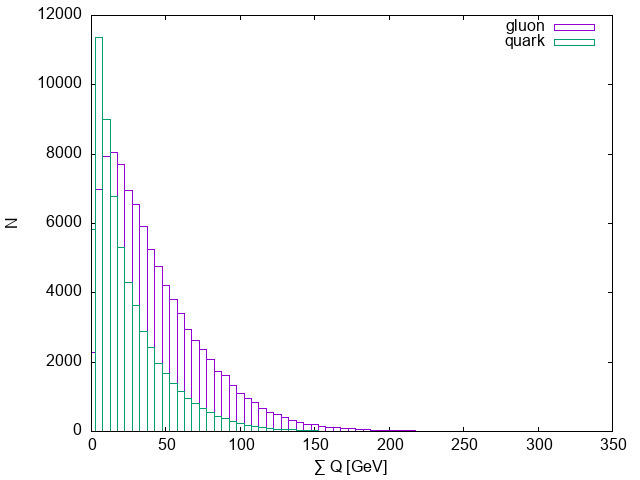
\includegraphics[width=.9\linewidth]{data_Q.png}
\end{center}


\begin{center}
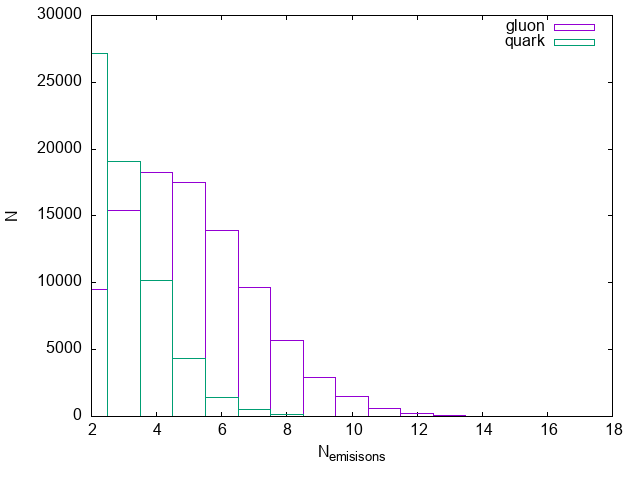
\includegraphics[width=.9\linewidth]{data_N.png}
\end{center}
\end{document}